% Springer LNCS manuscript -- generated draft, pending author verification.
% Compile with pdflatex (bibliography is inlined as thebibliography).
%
% REVISION 2026-09-09: rewritten after the isolated runs A/B/C. The earlier
% draft claimed format-biased verifiers CAUSE capability collapse. The
% single-variable control (Run B) refutes that claim. See
% papers/KET-QUA-CO-LAP-AC.md for the full data record and reasoning.
\documentclass[runningheads]{llncs}

\usepackage[T1]{fontenc}
\usepackage{graphicx}
\usepackage{booktabs}
\usepackage{amsmath}
\usepackage{array}
\usepackage{xcolor}
\usepackage{hyperref}
\renewcommand\UrlFont{\color{blue}\rmfamily}
\urlstyle{rm}

\begin{document}

\title{Verifier Bias Is Not Enough: A Controlled Re-examination of
Capability Collapse in Iterative Self-Training of Small Reasoning Models}

\titlerunning{Verifier Bias Is Not Enough}

\author{Tan Sang Nguyen\inst{1} \and Duy Anh Tran\inst{1}}
\authorrunning{T. S. Nguyen and D. A. Tran}
\institute{Ton Duc Thang University, Ho Chi Minh City, Vietnam\\
\email{52300057@student.tdtu.edu.vn, 52300006@student.tdtu.edu.vn}}

\maketitle

\begin{abstract}
Self-training loops (generate $\rightarrow$ verify $\rightarrow$ select
$\rightarrow$ train, GVT) assume a reliable verifier. We tested whether a
rule-based verifier with a directional format bias --- \texttt{math-verify}
rejects \verb|\dfrac|/\verb|\tfrac| rewrites of correct answers $100\%$ of the
time --- causes capability collapse over rounds. A pooled GSM8K\,+\,MATH-500 run
appeared to confirm it (Qwen2.5-1.5B pass@8 $72.6\%\to48.6\%$), but it shared one
adapter across datasets and scored on the selection items. With isolated
adapters, a held-out exam split and a matched patched-verifier control, the
collapse disappears at our training rate ($10^{-5}$) and patching changes nothing
across two paired seeds: the biased format is only $\approx0.55\%$ of generations,
so impact is severity $\times$ prevalence. A late check qualifies this: $10^{-5}$
barely trains the adapter. At $10^{-4}$ (one seed) the curves stay flat, but at
$5\times10^{-4}$ all four runs lose accuracy by round~2 and the drift grows with
the learning rate. The patch's effect flips sign between seeds, and no-filter and
train-on-gold controls show the verifier is not the driver. The decline has a
different anatomy in each regime: under self-training, generations that drift
and never answer rise from about $10\%$ to $40\%$ while accuracy on finished
solutions holds, only partly recovered by a larger token cap; under
reference-solution training, responses halve in length and accuracy truly falls.
A fixed token cap can thus turn a style change into an apparent loss of
reasoning.

\keywords{self-training \and verifier bias \and mathematical reasoning
\and small language models \and experimental confounds \and pass@k.}
\end{abstract}

\section{Introduction}
\label{sec:intro}

A common recipe for improving the mathematical reasoning of a small
language model (SLM) \emph{without additional human annotation} is to let
the model generate its own solutions, keep those that an automated
verifier judges correct, and fine-tune the model on the kept solutions,
repeating the process for several rounds. We refer to this recipe as the
\emph{Generate--Verify--Train} (GVT) loop. It underlies a family of
methods, including STaR~\cite{ref_star}, ReST~\cite{ref_rest} and
ReST-EM~\cite{ref_restem}, and rejection-sampling fine-tuning
(RFT)~\cite{ref_rft}. Its appeal is that the verifier plays the role of a
teacher that needs only to decide right from wrong; no reference solutions
are required.

Every method in this family rests on an implicit assumption: the verifier
separates correct from incorrect solutions reliably. This assumption is
routinely violated when the verifier is \emph{rule-based} --- the most
common choice for mathematics, because it is cheap, fast, and needs no
training of its own. A rule-based verifier such as
\texttt{math-verify}\footnote{\url{https://github.com/huggingface/math-verify},
version 0.9.0 with antlr4 4.13.2 in this work.}
extracts the final answer from a solution and compares it to the gold
answer after normalisation. It does not read the reasoning, and its
normalisation step never covers every equivalent way of writing an answer.
As a result it produces \emph{false negatives}: it rejects solutions that
are correct but written in a form it does not recognise. Crucially, this
error is \emph{directional}. Because the verifier compares an extracted
final answer against the gold, it almost never accepts a wrong answer --- a
false positive would require an incorrect answer that normalises exactly to
the gold, which is rare. Its errors are therefore overwhelmingly false
negatives, all pushing in one direction.

We measured this bias directly on \texttt{math-verify}
(Section~\ref{sec:verifier}). On GSM8K, whose answers are simple integers,
the false-negative rate on genuinely correct solutions is effectively
zero. On MATH-500, whose answers contain fractions and non-trivial
\LaTeX{}, it rises to roughly 7.8\%, and some individually valid rewrites
--- for instance writing \verb|\dfrac| instead of \verb|\frac| --- are
rejected 100\% of the time even though the numeric value is correct. The
bias is one-sided: we did not observe the verifier accepting incorrect
final answers.

This paper set out to ask a single question: \emph{when a directionally
biased verifier of this kind is used as the filter inside a GVT loop, and
the loop is run for many rounds rather than once, what is the consequence
--- does the model actually improve at reasoning, does it merely learn to
write in the style the verifier prefers, or does it lose capability?}

Our first experiments appeared to answer it decisively. Running five rounds
on a pooled GSM8K\,+\,MATH-500 set, both pass@1 and pass@8 fell sharply for
two model sizes, with the larger model collapsing harder. Taken at face
value this is a striking result, and an earlier version of this work
reported it as evidence that format-biased verifiers cause capability
collapse.

That conclusion does not survive a controlled re-examination, and reporting
why is the main contribution of this paper. The pooled design has two
properties that make it unable to answer the question it was built for.
First, it trains \emph{one shared} LoRA adapter each round on the union of
both datasets' accepted solutions, of which GSM8K supplies roughly $69\%$;
what happens on MATH-500 therefore cannot be separated from what happens on
GSM8K. Second, it evaluates on the same problems used to select training
data, so any round-over-round change mixes genuine capability change with
fit to the evaluation items. We rebuilt the experiment to remove both
properties --- one dataset per run, one adapter per dataset, and a held-out
$30\%$ exam split never used for selection --- and added the
single-variable control the original design lacked: an otherwise identical
MATH-500 run with the verifier's format bias patched.

Under the corrected design, the collapse largely disappears and the control
comes out null. Our own original hypothesis is not supported by the data
that were built to test it properly --- at the learning rate we used
($10^{-5}$), which a late diagnostic shows to be too low to train the
adapter; Section~\ref{sec:lrcheck} reports reruns at two higher rates. At
$10^{-4}$ the adapter trains and the curve stays flat; at $5\times10^{-4}$ it
does not, while the patch still shows no consistent effect, so we state the
flatness as conditional on the rate and the control as intact.

\paragraph{Contributions.}
\begin{itemize}
\item We characterise the directional bias of a real rule-based verifier
(\texttt{math-verify}) by format probe and by manual false-negative
audit, rather than simulating a noise model.
\item We run the GVT loop under two designs --- a \emph{pooled} design
representative of common practice, and an \emph{isolated} design with
per-dataset adapters and a held-out exam split --- and show that the two
give qualitatively different answers to the same question: dramatic
collapse under the first, essentially flat pass@8 under the second (at the
original learning rate; see Section~\ref{sec:lrcheck}).
\item We report the single-variable control that the pooled design could
not support: repairing the verifier's format bias, with everything else
held fixed, produces no measurable difference across two paired seeds at
the original learning rate. On
this evidence the hypothesis that directional verifier bias drives the
decline is \emph{not supported}.
\item We identify why, and argue the point generalises: the bias is severe
when triggered ($100\%$ rejection) but rare in practice (the affected
format appears in $\approx0.55\%$ of generations, and never on GSM8K).
Reported verifier-bias rates are conditional severities; their practical
impact is severity $\times$ prevalence, and prevalence must be measured in
the pipeline where the verifier will actually be used.
\item We decompose the decline that remains once these confounds are removed
and relate it to two recent studies (Section~\ref{sec:related}): under
self-training it is mostly generations that never finish, with accuracy on
finished ones unchanged; under reference-solution training it is shortened
responses and a real loss of accuracy.
\item We draw the methodological consequence: GVT-style experiments that
pool several datasets into one training mixture, or that score on the
selection set, can manufacture a collapse signal that isolation and
held-out evaluation do not reproduce.
\end{itemize}

\section{Related Work}
\label{sec:related}

\paragraph{Iterative self-training for reasoning.}
STaR~\cite{ref_star} introduced the generate--filter--retrain loop for
reasoning without hand-written rationales. ReST~\cite{ref_rest} and
ReST-EM~\cite{ref_restem} formalise it as alternating ``grow'' and
``improve'' steps; ReST-EM applies it to MATH and APPS with PaLM-2,
sampling 32 solutions per problem, and reports diminishing test gains after
the first round, plus a one-round regression on APPS that it does not
investigate. RFT~\cite{ref_rft} is the single-round rejection-sampling
special case. All of these treat the correctness signal as trustworthy;
none analyses a verifier that is biased in a fixed direction, and none
tracks output style across rounds.

\paragraph{Verifier and reward error.}
TinyV~\cite{ref_tinyv} measures that a rule-based verifier rejects a large
fraction of correct solutions and \emph{repairs} the verifier with an
auxiliary LLM check, evaluated in a single pass. From Accuracy to
Robustness~\cite{ref_robustness} reports that rule-based verifiers for
mathematical RL achieve only about 86\% recall on average (i.e.\ $\sim$14\%
false negatives), an independent figure consistent with ours, but runs RL
for a few hundred steps within one training phase and does not track how
verifier recall interacts with self-training rounds. Imperfect
Verifiers~\cite{ref_imperfect} gives the most formal noise model: the
verifier flips its decision with fixed probabilities $\rho_0$ (false
accept) and $\rho_1$ (false reject). Its Section~3.1 explicitly notes that
``real-world noise can depend on content, formatting, prompt style'', but
then assumes content-independent fixed rates and studies a single RL round.
Our study addresses the multi-round version of that gap; our answer, unlike
our initial expectation, is that a measured format-dependent bias of this
magnitude does not by itself change the multi-round outcome.

\paragraph{Limits of RL and self-training.}
Yue et al.~\cite{ref_rllimit} show that RL raises pass@1 while the base
model wins at large pass@$k$, i.e.\ RL sharpens an existing distribution
rather than extending capability. Teacher-Free
Self-Training~\cite{ref_teacherfree} runs three sequential self-training
rounds on a free-verifier domain and observes a pass@8 vs.\ pass@64
crossover --- the trained model wins at small sampling budget and loses at
large budget --- concluding that self-training ``amplifies but does not
compound''. Its verifier is exact string equality, with ``zero learned
opinion''. Our isolated runs are closer to this picture than to a collapse
picture: with the confounds removed, pass@8 is essentially preserved and
what erodes, mildly, is first-attempt reliability.

\paragraph{Model collapse.}
Training repeatedly on model-generated data erodes distribution tails and
converges output toward the mean~\cite{ref_collapse}. Qiao et
al.~\cite{ref_selectionbias} argue theoretically that a selector able to
``see'' only a narrow slice of the target distribution becomes itself a
source of bias that accelerates collapse. Our pooled runs looked like an
empirical instance of that mechanism; our isolated runs do not reproduce
it, which we read as a caution against inferring the mechanism from
aggregate pass-rate curves alone (Section~\ref{sec:discussion}).

\paragraph{Systematic verifier error.}
Egashira et al.~\cite{ref_delayplateau} classify verifier errors in RLVR on a
synthetic arithmetic task, with Qwen3-1.7B-Base and OLMo3-7B and
hand-designed error patterns such as format-based false negatives. They find
that systematic false negatives behave like random noise --- the model
learns to avoid the triggering output and still improves --- whereas
false positives can cause plateaus or collapse, and they note that real
verifiers may combine several failure modes. Our single-variable control
(Section~\ref{sec:control}) tests the same question in a different regime: a
\emph{real} verifier whose bias we measured, real GSM8K and MATH-500 data,
and several supervised self-training rounds instead of one RLVR phase. It
reaches the same conclusion they do.

\paragraph{Auditing self-improvement.}
Xu et al.~\cite{ref_phantom} audit three rounds of rank-32 LoRA
self-training of Qwen3-8B ($\eta=10^{-4}$, 256 problems per round; filters
by answer match, majority vote or an external teacher) against a frozen,
untrained control pushed through the same evaluation path. They identify
seven measurement failures, each of which inverts a reported finding when its
control is absent: a single greedy decode as the unit of measurement, an
expansion threshold whose null is non-zero, a fixed token cap under style
drift, training-seed variance (the corruption-to-learning ratio of one method
spans $0.55$--$1.53$ across seeds), and others. Substantively, self-training
does not improve rarely-solved problems ($0$--$2$ of $22$, against $8$--$11$
for distillation from a stronger teacher) and corrupts problems solved at
baseline well above their measured floor. This is the study closest to ours
in spirit, and our results meet theirs at three points: the A-versus-B gap
changes sign between seeds (their seed variance); a $150$-problem exam set
resolves only large effects (their low power of transition metrics); and
the self-training runs drift in style, which a fixed $512$-token cap may
then score as failure (Section~\ref{sec:anatomy}). The two studies are
complementary. They hold the filter and the learning rate fixed and use no
verifier whose format bias is measured; we vary the verifier and the
learning rate, compare pooled with isolated adapters, and add reference-solution
and no-filter controls, but we have no frozen control and no distillation arm.

\paragraph{Reference-guided training and response length.}
Kim et al.~\cite{ref_selfdistill} show that self-distillation, in which a
teacher copy of the model is conditioned on privileged information such as the
ground-truth solution, can cut mathematical accuracy by up to $40\%$
(Qwen3-1.7B/8B, DeepSeek-Distill-Qwen-7B, Olmo3-7B-Instruct) while
\emph{shortening} responses, which they trace to the suppression of epistemic
verbalization. Our train-on-gold control (Section~\ref{sec:lrcheck}) is a
supervised, small-model analogue and shows the same signature: mean response
length falls by $59\%$ ($1{,}175\to485$ characters) and accuracy on completed
solutions falls from $37\%$ to $14\%$. We did not measure epistemic markers,
and Qwen2.5-Instruct is not a long-chain-of-thought model, so we claim the
signature, not the mechanism. The same figure shows the \emph{opposite} length
drift under self-training (Section~\ref{sec:anatomy}), which this literature
does not predict.

\paragraph{Summary.}
In the literature we surveyed (searched through October 2026) we found no
study that combines a real, measured, format-biased rule-based verifier with
several sequential self-training rounds and a matched patched-verifier
control. The closest are Egashira et al.\ (hand-designed errors, one RLVR
phase) and Xu et al.\ (a measurement audit with answer, vote and teacher
filters). We add that combination, a design-level account of how pooled
adapters, selection-set scoring and an undertrained adapter each manufacture a
misleading curve, and a decomposition of the decline that remains once they are
removed. The answer to the verifier question is negative: within our
measurement precision, the bias does not change the multi-round outcome.

\section{Setup}
\label{sec:setup}

\subsection{The GVT Loop}
\label{sec:loop}

Each round $t$ of our loop performs four steps.
\begin{description}
\item[Generate.] For every problem in the working set, the current model
samples $k = 8$ solutions (temperature sampling).
\item[Verify.] \texttt{math-verify} (version 0.9.0, antlr4 4.13.2) extracts
the final answer from each solution and compares it to the gold answer.
\item[Select.] Solutions the verifier accepts are kept; all others are
discarded.
\item[Train.] A \emph{fresh} LoRA adapter (rank 16, $\alpha = 32$) is
attached to the \emph{base} model and trained by supervised fine-tuning on
the kept solutions for one epoch. Adapters are \emph{not} accumulated
across rounds: round $t$ starts from the base weights and learns only from
round $t-1$'s accepted pool.
\end{description}
The loop is run for five rounds ($t = 0,\dots,4$), where $t = 0$ is the
untrained base model.

\subsection{The Verifier and Its Directional Bias}
\label{sec:verifier}

Before running the loop we characterised \texttt{math-verify} in two ways.

\emph{Format probe.} We took gold answers from GSM8K and MATH-500 and
re-rendered each in a set of individually valid formats (bare number,
trailing-zero decimal, \verb|\frac|, \verb|\dfrac|, \verb|\tfrac|, boxed,
dollar-delimited, full sentence, with units), then asked the verifier to
grade the re-rendered answer against the original gold. On GSM8K, plain
rewrites are never rejected; \verb|\dfrac| and \verb|\tfrac| are rejected
$200/200$ (the verifier fails to parse the command). On MATH-500,
\verb|\dfrac|/\verb|\tfrac| are rejected $146/146$ ($100\%$),
trailing-zero decimals such as \texttt{0.50} are rejected $59\%$ of the
time, and boxed/dollar-delimited forms are rejected about $20\%$ of the
time.

\emph{False-negative rate on real solutions.} We then took genuinely
correct model-generated solutions (public teacher traces for GSM8K; public
Qwen2.5-7B rollouts for MATH-500) and manually checked, for each solution
the verifier rejected, whether the boxed answer actually matched the gold.
The false-negative rate among correct solutions is $\mathbf{7.8\%}$ on
MATH-500 ($10/128$) and $\mathbf{0\%}$ on GSM8K ($0/200$); the two verifier
presets we tested (\texttt{default} and \texttt{reward}) give identical
counts. Of the ten MATH-500 false negatives, eight are cases where the
verifier extracts the wrong token from a long solution, and two are valid
rewrites it cannot match (\verb|\left( 3, \frac{\pi}{2} \right)| vs.\
\verb|(3, \frac{\pi}{2})|; \verb|6+9i| vs.\ \verb|6 + 9i|). We did not
observe the verifier accepting an incorrect final answer; the error is
one-directional.

\emph{The patch.} For the control experiment we repaired exactly the
largest identified failure mode: a normalisation pass that rewrites
\verb|\dfrac| and \verb|\tfrac| to \verb|\frac| before the verifier's own
parsing. This removes the $100\%$-rejection format class from the
verifier's error profile while leaving every other behaviour untouched.

\subsection{Two Experimental Designs}
\label{sec:designs}

Our results come from two designs, summarised in
Table~\ref{tab:designs}. The distinction is the central point of this
paper, so we state it explicitly rather than as a configuration detail.

\emph{Design~P (pooled).} Both datasets are loaded together, and each round
trains \emph{one} LoRA adapter on the union of the accepted solutions from
both. Selection and evaluation use the same problems. This is the design
of our initial experiments and, in structure, of much reported practice.

\emph{Design~I (isolated).} One dataset per run, one adapter per run, and a
held-out split: $30\%$ of the problems ($150$ of $500$) form an
\texttt{exam} set that is \emph{never} used to select training data, while
the remaining $350$ form the \texttt{select} set. All reported pass rates
under Design~I are computed on the held-out exam set only.

\begin{table}[t]
\caption{The two designs. Design~I removes the pooling confound and the
selection/evaluation overlap, and adds the patched-verifier control.}
\label{tab:designs}
\centering
\begin{tabular}{lll}
\toprule
& Design~P (pooled) & Design~I (isolated) \\
\midrule
Datasets per run & GSM8K + MATH-500 & one only \\
Adapter & one, shared & one per dataset \\
Training mixture & $\approx$\,69\% GSM8K & single-domain \\
Evaluation items & same as selection & held-out 30\% \\
Verifier control & none & Run~B (patched) \\
Models & 0.5B and 1.5B & 1.5B \\
Runs & 2 & 3 (A, B, C) \\
\bottomrule
\end{tabular}
\end{table}

Design~I comprises three runs, all Qwen2.5-1.5B-Instruct, $n=500$,
five rounds, $k=8$, \texttt{holdout-frac}~$=0.3$, seed~$0$, differing in
exactly one respect each:
\begin{description}
\item[Run A.] MATH-500 only, original verifier. The dataset where the bias
is present, isolated.
\item[Run B.] MATH-500 only, \emph{patched} verifier. Identical to Run~A in
every other respect; the single-variable control for the paper's central
hypothesis.
\item[Run C.] GSM8K only, original verifier. The dataset where the verifier
is already near-clean ($0\%$ measured false negatives).
\end{description}
Run~A was additionally repeated with seed~$1$. Because the seed governs the
train/exam partition as well as sampling, the repetition draws a
\emph{different} 150-problem exam set, which lets us calibrate how much of
any observed movement is attributable to the choice of evaluation items
(Section~\ref{sec:seedvar}).

\subsection{Models, Data, Training, Metrics}
\label{sec:config}

\emph{Models.} Qwen2.5-0.5B-Instruct and
Qwen2.5-1.5B-Instruct.\footnote{\url{https://huggingface.co/Qwen/Qwen2.5-0.5B-Instruct},
\url{https://huggingface.co/Qwen/Qwen2.5-1.5B-Instruct}.}
Design~P uses both; Design~I uses the 1.5B model only.

\emph{Data.} GSM8K~\cite{ref_gsm8k} and MATH-500 --- the 500-problem
subset of MATH~\cite{ref_math} --- 500 problems each, drawn from the test
splits.

\emph{Training.} LoRA supervised fine-tuning
(\texttt{transformers} + \texttt{peft} + TRL \texttt{SFTTrainer}), one
epoch per round at a learning rate of $10^{-5}$ in every run reported
here.\footnote{A post-hoc diagnostic indicates this rate undertrains the
adapter (Limitation~1).}
We use SFT on verifier-accepted solutions rather than
online RL because it matches the select-then-train structure of the loop.

\emph{Metrics, per round.}
(i) pass@1 and pass@8;
(ii) style counts over all generations in the round, for labels including
\texttt{boxed}, \texttt{dfrac}, \texttt{frac}, \texttt{dollar},
\texttt{sentence}, \texttt{assignment}, \texttt{decimal};
(iii) pre-filter answer diversity: the mean fraction of distinct normalised
final answers among the $k$ samples for a problem, and the fraction of
problems on which all $k$ samples agree;
(iv) for Design~I, the final training loss reported by
\texttt{SFTTrainer} on that round's kept pool.

\emph{Infrastructure.} A single Kaggle T4 GPU. Design~P and Run~C were run
once; Runs~A and~B were run at two seeds (Section~\ref{sec:seedvar} and
Section~\ref{sec:limitations}).

\section{Results}
\label{sec:results}

\subsection{Design P: An Apparent Collapse}
\label{sec:pooled}

Table~\ref{tab:passk} reports pass@1 and pass@8 for both models across the
five rounds of the pooled design; the two verifier presets produced
identical values, so a single column is shown. All four series decline
monotonically or nearly so (the only exception is a $+0.8$-point blip in
0.5B pass@1 at round~1), and the 1.5B decline is severe and accelerating.

\begin{table}[t]
\caption{Design~P: pass@1 and pass@8 over five GVT rounds, pooled
GSM8K + MATH-500, scored on the selection set. Round 0 is the untrained
base model. Section~\ref{sec:confound} explains why these numbers cannot
be attributed to verifier bias.}
\label{tab:passk}
\centering
\begin{tabular}{llccccc c}
\toprule
Model & Metric & R0 & R1 & R2 & R3 & R4 & $\Delta$ (R0$\to$R4) \\
\midrule
0.5B & pass@1 & 31.1\% & 31.9\% & 29.9\% & 28.9\% & 27.4\% & $-3.7$ pt \\
0.5B & pass@8 & 60.5\% & 58.9\% & 56.1\% & 55.5\% & 54.9\% & $-5.6$ pt \\
1.5B & pass@1 & 50.0\% & 46.2\% & 44.5\% & 32.4\% & 18.6\% & $\mathbf{-31.4}$ pt \\
1.5B & pass@8 & 72.6\% & 71.5\% & 70.2\% & 63.6\% & 48.6\% & $\mathbf{-24.0}$ pt \\
\bottomrule
\end{tabular}
\end{table}

\begin{figure}[t]
\centering
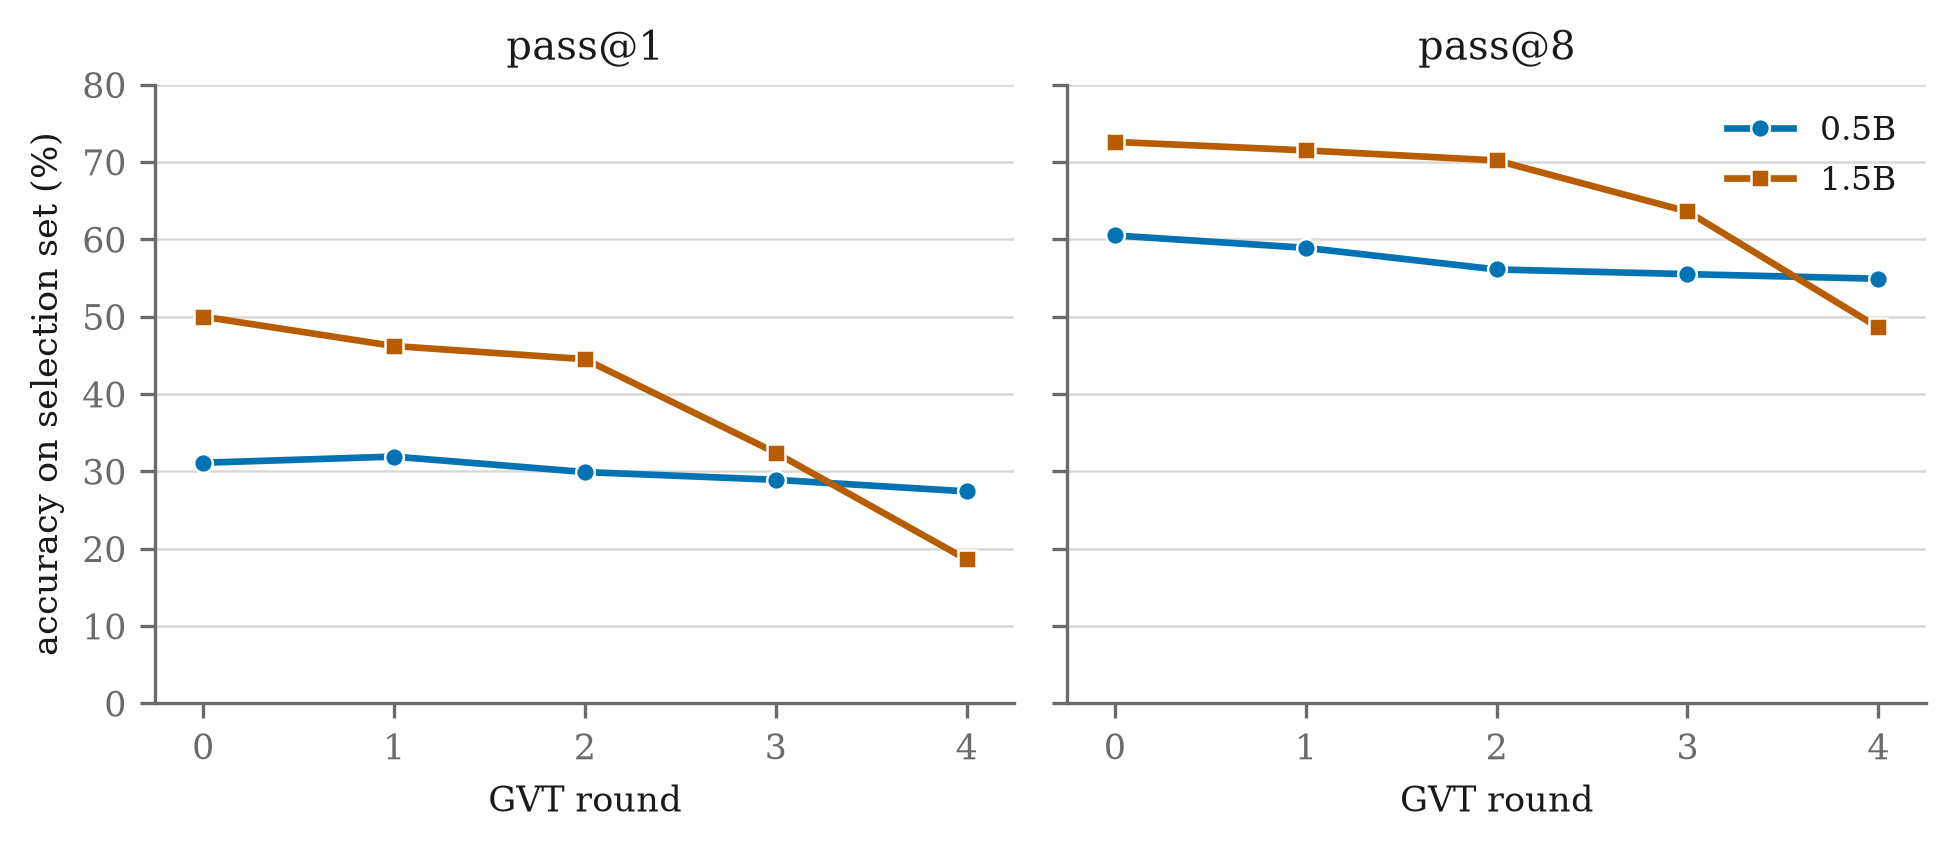
\includegraphics[width=\textwidth]{pass_at_k_by_round.png}
\caption{Design~P: pass@1 and pass@8 across five rounds for both model
sizes. Both metrics fall for both models. Section~\ref{sec:isolated} shows
that this pattern does not survive isolation and held-out evaluation.}
\label{fig:passk}
\end{figure}

Splitting the 1.5B pooled run by dataset (Table~\ref{tab:bydataset})
sharpens the puzzle rather than resolving it. Under the original
hypothesis, MATH-500 --- where the verifier's false-negative rate is
$7.8\%$ --- should degrade and GSM8K --- where it is $0\%$ --- should hold
steady. Instead both fall heavily, and GSM8K, the dataset with the clean
verifier, loses more pass@1 in absolute points than MATH-500.

\begin{table}[t]
\caption{Design~P, 1.5B, split by dataset. GSM8K has a measured $0\%$
verifier false-negative rate yet declines at least as much as MATH-500.}
\label{tab:bydataset}
\centering
\begin{tabular}{llccccc c}
\toprule
Dataset & Metric & R0 & R1 & R2 & R3 & R4 & $\Delta$ \\
\midrule
GSM8K & pass@1 & 69.6\% & 62.0\% & 61.0\% & 45.6\% & 26.6\% & $-43.0$ pt \\
GSM8K & pass@8 & 91.4\% & 90.4\% & 89.0\% & 82.2\% & 65.8\% & $-25.6$ pt \\
MATH-500 & pass@1 & 30.4\% & 30.4\% & 28.0\% & 19.2\% & 10.6\% & $-19.8$ pt \\
MATH-500 & pass@8 & 53.8\% & 52.6\% & 51.4\% & 45.0\% & 31.4\% & $-22.4$ pt \\
\bottomrule
\end{tabular}
\end{table}

The accepted training pool also contracts every round --- mildly for the
0.5B model ($-16\%$ by round~4) and sharply for the 1.5B model ($-60\%$,
from $3{,}962$ to $1{,}566$ solutions) --- and 1.5B output style shifts
markedly, with \verb|\boxed{}| occurrences falling from $5{,}608$ to
$2{,}693$ while dollar-delimited math rises from $1{,}453$ to $3{,}406$.
Read on its own, this is a coherent story about a shrinking, style-skewed
pool driving capability down.

\subsection{Why Design P Cannot Answer the Question}
\label{sec:confound}

Two properties of Design~P block the inference.

\emph{Shared adapter over a pooled mixture.} Each round trains one adapter
on the union of both datasets' accepted solutions.
Table~\ref{tab:poolmix} shows the composition of that union: GSM8K supplies
between $68.4\%$ and $70.2\%$ of it in every round. The adapter evaluated
on MATH-500 is therefore one that learned roughly $69\%$ of its update
signal from GSM8K, and vice versa. Whatever happens to either dataset's
score is a joint function of both datasets' filtered pools, and no
contrast within this design isolates the verifier's contribution. We note
that the mixture ratio is \emph{stable} across rounds, which rules out a
drifting-ratio explanation but does not remove the interference itself.

\begin{table}[t]
\caption{Design~P, 1.5B: composition of the shared training pool. GSM8K
dominates the mixture in every round, so neither dataset's trajectory is
independent of the other.}
\label{tab:poolmix}
\centering
\begin{tabular}{lccccc}
\toprule
Round & 0 & 1 & 2 & 3 & 4 \\
\midrule
Kept, GSM8K & 2725 & 2551 & 2356 & 1837 & 1100 \\
Kept, MATH-500 & 1237 & 1179 & 1039 & 800 & 466 \\
GSM8K share & 68.8\% & 68.4\% & 69.4\% & 69.7\% & 70.2\% \\
\bottomrule
\end{tabular}
\end{table}

\emph{Selection and evaluation on the same problems.} Design~P scores each
round on the problems it also used to choose training data. A round-over-round
change therefore mixes capability change with fit to those specific items,
and neither component can be recovered from the aggregate.

\begin{figure}[t]
\centering
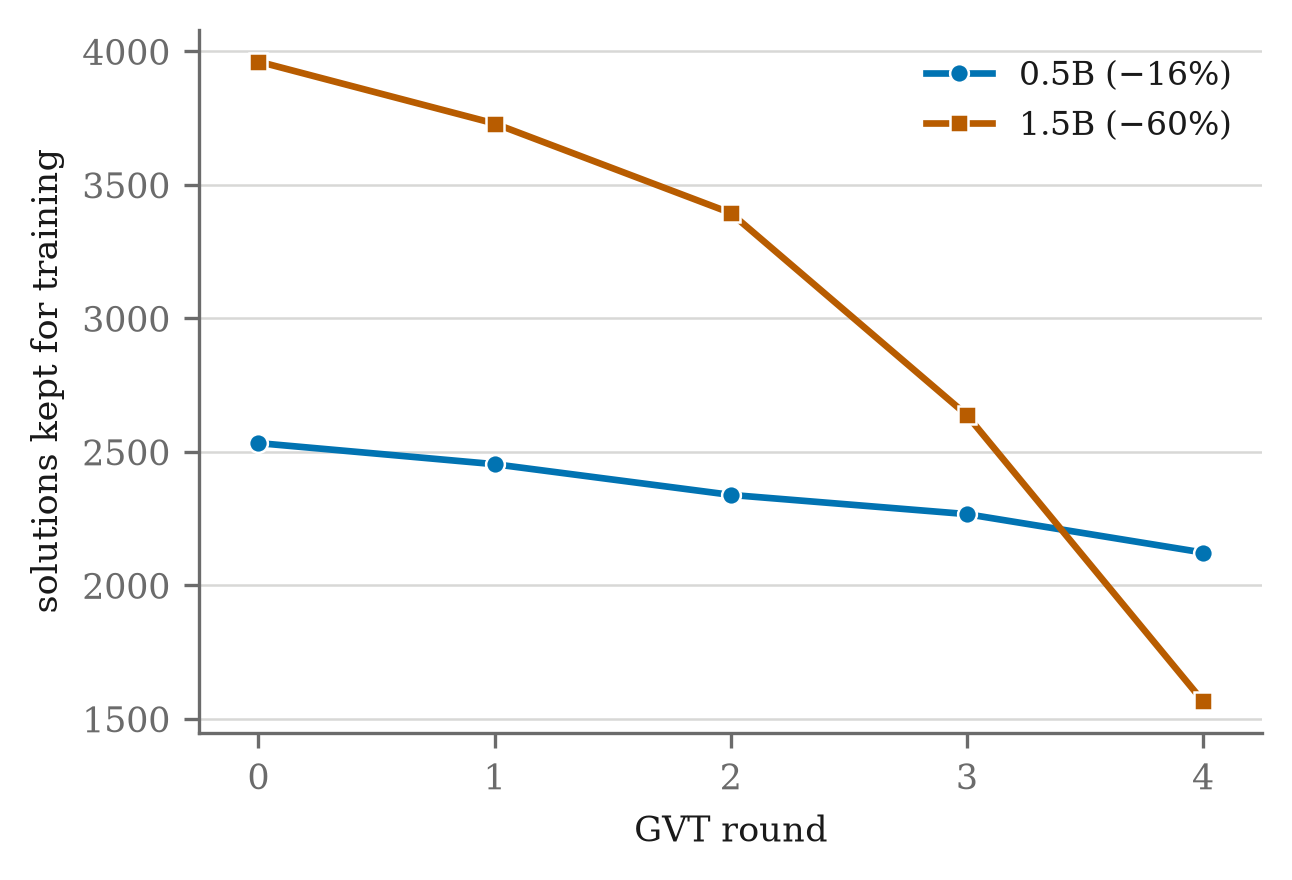
\includegraphics[width=\textwidth]{selected_pool_by_round.png}
\caption{Design~P: size of the verifier-accepted training pool by round.
The pool contracts in both runs. Section~\ref{sec:isolated} shows pool
contraction also occurs \emph{without} a corresponding pass@8 decline,
which weakens the shrinking-pool explanation.}
\label{fig:pool}
\end{figure}

\subsection{Design I: The Collapse Does Not Reproduce at the Original Learning Rate}
\label{sec:isolated}

Table~\ref{tab:isolated} reports the isolated runs on their held-out exam
sets. The severe collapse of Table~\ref{tab:passk} is absent. pass@8 is
flat in every run: $57.3\%\to56.0\%$ and $58.7\%\to58.7\%$ for Run~A at
seeds 0 and 1, $57.3\%\to53.3\%$ for Run~B, and $92.7\%\to90.0\%$ for
Run~C, against declines of $22$--$26$ points in the pooled design. On
MATH-500 --- the dataset the hypothesis is about --- pass@1 falls by about
three points at round~1 and is flat thereafter, and the two seeds of Run~A
agree on this shape ($-2.7$ and $-3.4$ points end to end).

The shape itself is informative, and having two seeds is what makes it
readable. In both, essentially the entire pass@1 movement occurs at
round~1 ($32.0\to29.3$ at seed~0; $36.7\to32.7$ at seed~1), after which
rounds 1--4 show no trend in either direction ($29.3, 28.0, 29.3, 29.3$ and
$32.7, 32.7, 31.3, 33.3$). This is a one-off cost of the first
self-training round rather than a compounding process --- which is the
signature the collapse hypothesis predicts and does not find here. It
matches the ``amplifies but does not compound'' reading
of~\cite{ref_teacherfree} more closely than any collapse account.

\begin{table}[t]
\caption{Design~I: pass@1 and pass@8 on the held-out exam set (150
problems), Qwen2.5-1.5B. Runs A and B differ only in whether the verifier's
format bias is patched. Run~A is shown for both seeds; seed~1 draws a
different exam partition, so its round-0 value differs
(Section~\ref{sec:seedvar}).}
\label{tab:isolated}
\centering
\begin{tabular}{llccccc c}
\toprule
Run & Metric & R0 & R1 & R2 & R3 & R4 & $\Delta$ \\
\midrule
A, seed 0 (MATH-500, orig.) & pass@1 & 32.0\% & 29.3\% & 28.0\% & 29.3\% & 29.3\% & $-2.7$ pt \\
A, seed 0 (MATH-500, orig.) & pass@8 & 57.3\% & 56.7\% & 54.7\% & 57.3\% & 56.0\% & $-1.3$ pt \\
A, seed 1 (MATH-500, orig.) & pass@1 & 36.7\% & 32.7\% & 32.7\% & 31.3\% & 33.3\% & $-3.4$ pt \\
A, seed 1 (MATH-500, orig.) & pass@8 & 58.7\% & 60.7\% & 59.3\% & 59.3\% & 58.7\% & $\phantom{-}0.0$ pt \\
B, seed 0 (MATH-500, patched) & pass@1 & 32.0\% & 28.7\% & 28.7\% & 28.7\% & 28.7\% & $-3.3$ pt \\
B, seed 0 (MATH-500, patched) & pass@8 & 57.3\% & 55.3\% & 52.0\% & 57.3\% & 53.3\% & $-4.0$ pt \\
B, seed 1 (MATH-500, patched) & pass@1 & 37.3\% & 32.0\% & 32.7\% & 31.3\% & 33.3\% & $-4.0$ pt \\
B, seed 1 (MATH-500, patched) & pass@8 & 59.3\% & 60.7\% & 58.0\% & 58.7\% & 58.7\% & $-0.6$ pt \\
C, seed 0 (GSM8K, orig.) & pass@1 & 66.7\% & 66.7\% & 65.3\% & 63.3\% & 54.0\% & $-12.7$ pt \\
C, seed 0 (GSM8K, orig.) & pass@8 & 92.7\% & 90.7\% & 93.3\% & 90.0\% & 90.0\% & $-2.7$ pt \\
\bottomrule
\end{tabular}
\end{table}

\begin{figure}[t]
\centering
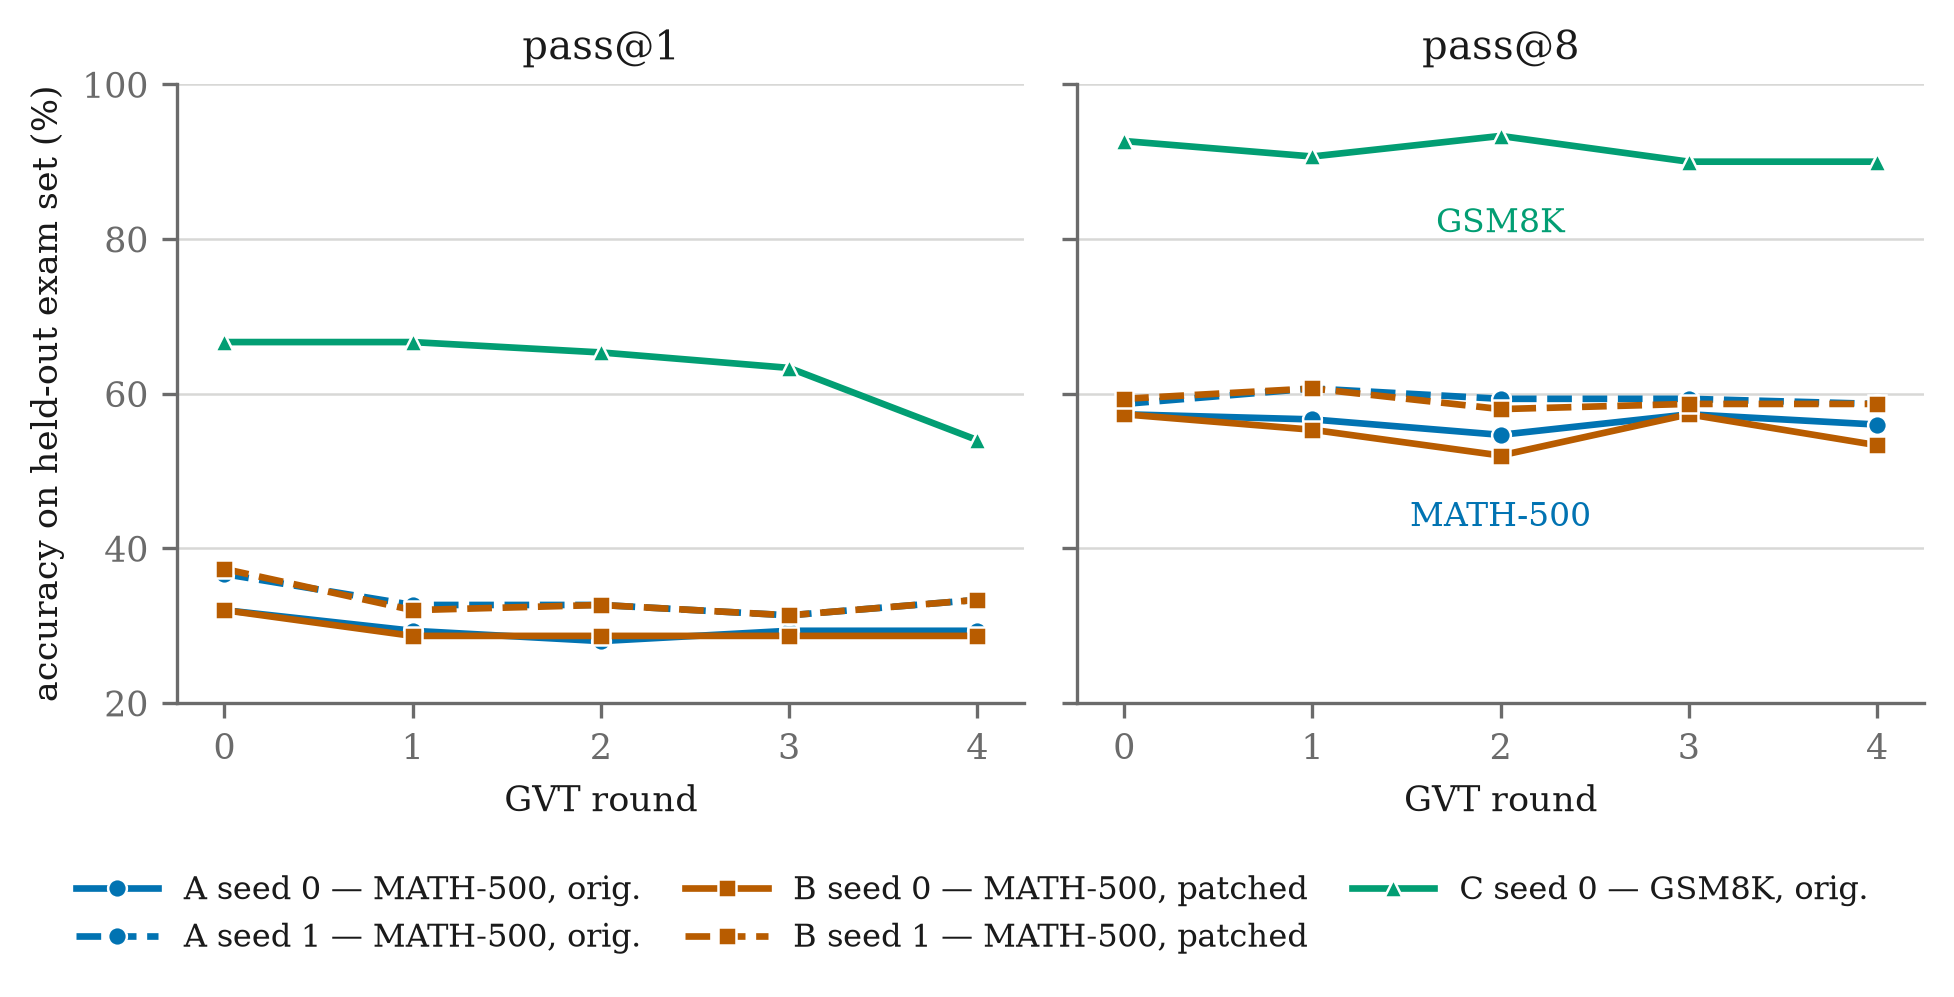
\includegraphics[width=\textwidth]{isolated_by_round.png}
\caption{Design~I: pass@1 (left) and pass@8 (right) on the held-out exam
set, by round. Colour identifies the run, line style the seed, marker the
run again, so the figure survives greyscale printing. Runs A and B ---
identical except for the verifier patch --- track each other closely at both
seeds. pass@8 is flat in every run, in contrast to the $22$--$26$ point
declines of Design~P (Fig.~\ref{fig:passk}). The one visible movement is
Run~C's pass@1 in the final round.}
\label{fig:isolated}
\end{figure}

Figure~\ref{fig:isolated} plots the same data. Run~C retains a residual
effect worth naming: GSM8K pass@1 falls $12.7$
points while its pass@8 does not move. The model does not lose the ability
to reach a correct answer within eight attempts; it becomes less reliable
at producing one on the first. Almost the entire drop occurs in the final
round ($63.3\%\to54.0\%$), and with a $150$-problem exam set and a single
seed we cannot presently separate this from noise. We flag it as the one
open empirical question these runs leave behind, not as a finding.

The accepted pools under Design~I contract as well --- Run~C from $1{,}901$
to $1{,}515$ kept solutions ($-20\%$), Run~A from $872$ to $843$
($-3\%$) --- yet pass@8 in both runs is flat. Pool contraction and
capability collapse, which moved together in Design~P, come apart here.

\subsection{Calibrating the Noise Floor}
\label{sec:seedvar}

The two seeds of Run~A also give us something the study previously lacked:
a measured scale for how large a difference must be before it means
anything. Round~0 is the \emph{untrained base model}, identical in both
seeds; the only thing that differs is which 150 problems the seed assigned
to the exam partition. Yet round~0 pass@1 is $32.0\%$ at seed~0 and
$36.7\%$ at seed~1 --- a gap of $4.7$ points, or seven problems --- with
pass@8 differing by $1.4$ points.

The figure is worth stating precisely, because it is easy to misuse. It is
a \emph{between-partition} variance, and most of the comparisons this paper
relies on are \emph{within}-partition and therefore paired: round~0 versus
round~4 inside one run scores the same 150 problems, and Runs A and B at
seed~0 share a partition. In those paired comparisons the partition
variance largely cancels, so $4.7$ points is not an error bar for them. It
does bound a different and equally important thing: any comparison of
\emph{absolute} levels across runs with different seeds --- for instance
Run~A's $32.0\%$ at seed~0 against $36.7\%$ at seed~1 --- carries several
points of partition noise and should not be read as an effect.

With that stated, the number still does useful work. It shows that a
$150$-problem exam set resolves differences of a few points only weakly,
which is the regime the A-versus-B gap of $0.6$ points sits in; and it puts
the Run~C decline of $12.7$ points comfortably outside the range that
partition choice alone can explain.

\subsection{The Control: Patching the Verifier Changes Nothing at the Original Rate}
\label{sec:control}

Runs A and B are identical in dataset, seed, split, model, and training
configuration, and differ only in whether \verb|\dfrac|/\verb|\tfrac| are
normalised before verification --- the one error class we measured at
$100\%$ rejection. This is the single-variable control the paper's central
hypothesis requires, and which Design~P could not provide.

The two curves are indistinguishable at our measurement precision
(Table~\ref{tab:isolated}). Over five rounds pass@1 ends at $29.3\%$
unpatched versus $28.7\%$ patched --- a difference of $0.6$ points, i.e.\
one problem out of $150$ --- and pass@8 at $56.0\%$ versus $53.3\%$, with
Run~B's pass@8 oscillating non-monotonically ($55.3\to52.0\to57.3\to53.3$)
in a manner consistent with sampling noise rather than a trend. Pre-filter
answer diversity is likewise near-identical between the two
(Table~\ref{tab:answer-diversity}), as are their per-round training losses
($0.38\to0.43$ for A, $0.39\to0.44$ for B).

The pattern repeats at seed~1, where the agreement is closer still: from
round~2 onward the two runs report \emph{identical} pass@1
($32.7\%$, $31.3\%$, $33.3\%$), and their end-to-end changes are $-3.4$
versus $-4.0$ points. Across both seeds, no round shows a difference larger
than $2.7$ points in pass@1, and the differences have no consistent sign.

Repairing the verifier's measured format bias produces no measurable
improvement. Within the precision of this experiment --- now two paired
seeds --- the hypothesis that directional format bias in the verifier
drives multi-round degradation is \emph{not supported}.
Section~\ref{sec:prevalence} explains why.

\subsection{Why the Patch Does Nothing: Severity Without Prevalence}
\label{sec:prevalence}

A null result is more useful when the mechanism behind it is identified,
and our style counts supply one directly.

Round~0 gives an unusually clean measurement. At a fixed seed, Runs A and B
generate from the same base model with the same sampling seed and have not
yet trained on anything, so their round-0 generations are identical --- the
style counts confirm this exactly (e.g.\ $29$ \verb|\dfrac| occurrences in
both runs at seed~1). The \emph{only} difference at round~0 is which
verifier scores those identical solutions. The patch's direct scoring
effect is therefore isolated with no confounds at all, and it is: zero
problems out of $150$ at seed~0 ($32.0\%$ both), and one problem out of
$150$ at seed~1 ($36.7\%$ versus $37.3\%$).

The reason is prevalence. Table~\ref{tab:prevalence} counts how often the
patched format class actually occurs in the model's output. Across $4{,}000$
generations per round on MATH-500, \verb|\dfrac| appears in $20$--$29$ of
them --- about $0.55\%$ --- and \verb|\tfrac| never appears at all. On
GSM8K, whose answers are integers, \verb|\dfrac| occurs zero times in every
round, which is why no patched GSM8K run is worth spending compute on.

\begin{table}[t]
\caption{Occurrences of the patched format class among the $4{,}000$
generations produced per round. The bias is severe when triggered
($100\%$ rejection, Section~\ref{sec:verifier}) but is triggered rarely.}
\label{tab:prevalence}
\centering
\begin{tabular}{llccccc}
\toprule
Dataset & Token & R0 & R1 & R2 & R3 & R4 \\
\midrule
MATH-500 & \verb|\dfrac| & 23--29 & 23 & 22 & 21--22 & 20--22 \\
MATH-500 & \verb|\tfrac| & 0 & 0 & 0 & 0 & 0 \\
GSM8K & \verb|\dfrac| & 0 & 0 & 0 & 0 & 0 \\
GSM8K & \verb|\tfrac| & 0 & 0 & 0 & 0 & 0 \\
\bottomrule
\end{tabular}
\end{table}

This resolves an apparent tension in our own measurements. The format probe
of Section~\ref{sec:verifier} reports $100\%$ rejection for
\verb|\dfrac|/\verb|\tfrac|, which sounds severe, but it measures severity
\emph{conditional on the format occurring}. The quantity that governs the
training pool is severity $\times$ prevalence: $100\%$ of $0.55\%$ is
$0.55\%$ of solutions wrongly discarded per round. A pool reduced by half a
percent cannot plausibly drive a twenty-point capability change. Our own
false-negative audit points the same way in retrospect: of the ten
MATH-500 false negatives we found, only two were format rewrites, while
eight were wrong-token extraction from long solutions --- a failure mode the
patch does not address.

We think this is the most transferable lesson of the study. Verifier-bias
figures in the literature, including the $\sim$14\% false-negative rate
of~\cite{ref_robustness} and the large rejected fractions
of~\cite{ref_tinyv}, are conditional severity figures measured on some
reference distribution. Whether such a bias matters in a given pipeline
depends on how often the affected forms appear in \emph{that pipeline's}
model output, which is a cheap thing to count and which we did not count
until after the hypothesis had failed.

\subsection{Pre-Filter Answer Diversity Increases, It Does Not Collapse}
\label{sec:answer-diversity}

A natural companion question is whether the model converges onto a single
\emph{answer} per problem --- whether the $k$ raw samples for one problem,
\emph{before} the verifier sees them, become more alike as training
proceeds. We measured this in both designs by extracting each sample's
final answer and computing, per round, the mean fraction of distinct
normalised answers among the $k=8$ samples and the fraction of problems on
which all $k$ agree.

\begin{table}[t]
\caption{Pre-filter answer diversity across $k{=}8$ samples per problem, by
round. A \emph{lower} ``\% all-$k$ agree'' means the model is \emph{less}
consistent about what answer it gives to the same problem.}
\label{tab:answer-diversity}
\centering
\begin{tabular}{lccccc}
\toprule
Run / metric & R0 & R1 & R2 & R3 & R4 \\
\midrule
\multicolumn{6}{l}{\emph{Design~P}} \\
0.5B, unique answers / $k$ & 0.600 & 0.601 & 0.608 & 0.620 & 0.649 \\
0.5B, \% all-$k$ agree & 10.5\% & 10.8\% & 9.2\% & 9.1\% & 7.3\% \\
1.5B, unique answers / $k$ & 0.443 & 0.482 & 0.543 & 0.634 & 0.712 \\
1.5B, \% all-$k$ agree & \textbf{24.8\%} & 21.4\% & 14.5\% & 6.6\% & \textbf{1.7\%} \\
\midrule
\multicolumn{6}{l}{\emph{Design~I}} \\
A (seed 0), unique answers / $k$ & 0.542 & 0.545 & 0.545 & 0.546 & 0.554 \\
A (seed 0), \% all-$k$ agree & 14.6\% & 13.4\% & 13.2\% & 12.2\% & 12.0\% \\
A (seed 1), unique answers / $k$ & 0.528 & 0.539 & 0.548 & 0.543 & 0.549 \\
A (seed 1), \% all-$k$ agree & 16.0\% & 15.2\% & 13.2\% & 13.8\% & 12.6\% \\
B (seed 0), unique answers / $k$ & 0.542 & 0.546 & 0.545 & 0.547 & 0.555 \\
B (seed 0), \% all-$k$ agree & 14.6\% & 13.8\% & 14.2\% & 12.2\% & 12.2\% \\
B (seed 1), unique answers / $k$ & 0.528 & 0.542 & 0.544 & 0.545 & 0.543 \\
B (seed 1), \% all-$k$ agree & 16.0\% & 15.2\% & 14.0\% & 13.2\% & 12.8\% \\
C, unique answers / $k$ & 0.359 & 0.364 & 0.413 & 0.444 & 0.500 \\
C, \% all-$k$ agree & 33.6\% & 32.4\% & 25.2\% & 18.8\% & 16.0\% \\
\bottomrule
\end{tabular}
\end{table}

In both designs, answer-level diversity \emph{rises} --- the opposite of a
``the model narrows onto one preferred output'' picture. (Raw-text
uniqueness among the $k$ samples stays at $\approx\!1.0$ every round: at
temperature $0.8$, independent samples are almost never byte-identical, so
that metric is uninformative here.) The magnitude tracks the magnitude of
the pass@1 decline: steep in Design~P's 1.5B run ($24.8\%\to1.7\%$ all-$k$
agreement), moderate in Run~C ($33.6\%\to16.0\%$), and nearly flat in Runs
A and B, which are also the runs whose pass@1 barely moves. This is
consistent with a single underlying quantity --- first-attempt reliability
--- rather than with stylistic convergence: a model that still solves a
problem tends to land on the same answer across attempts, while one whose
reliability is eroding answers more erratically, which depresses pass@1
while leaving pass@8 comparatively intact.

\subsection{A Learning-Rate Check: The Flatness Is Conditional}
\label{sec:lrcheck}

Every run above used a LoRA learning rate of $10^{-5}$. A one-round diagnostic
on the same MATH-500 pool (Limitation~1) shows that rate barely trains the
adapter: training loss oscillates between $0.68$ and $0.84$ with no downward
trend, against a fall to $0.24$--$0.28$ at $5\times10^{-4}$. The flat curves
of Design~I, and the null control, could therefore reflect a training step
that hardly moves the model. We reran Run~A and its matched control Run~B
(verifier patched) at $5\times10^{-4}$ at two seeds, changing nothing else
except two compute-driven reductions: three rounds instead of five, and $k=4$
samples per problem instead of $8$ (so pass@4 replaces pass@8). Seed~1 uses
the same exam partition as the seed-1 runs above; seed~2 draws a new one. The
round-0 values differ from the earlier runs' only through sampling, since all
score the untrained base model. These are the first runs in this study whose
adapter measurably fits its data: the loss falls from about $0.5$ to $0.25$
within round~0. A later run of A at an intermediate rate, $10^{-4}$ (seed~1,
same partition), fills in the middle of the range.

\begin{table}[t]
\caption{Runs A and B rerun at $5\times10^{-4}$, and Run~A at $10^{-4}$ (last
block) (MATH-500, $k=4$, three rounds), held-out exam set of 150 problems. B differs from A only in the
verifier patch; each seed draws its own exam partition. ``Boxed'' is the share
of the $2{,}000$ generations in each round containing
\texttt{\textbackslash boxed}.}
\label{tab:lrcheck}
\centering
\setlength{\tabcolsep}{6pt}
\begin{tabular}{lcccccc}
\toprule
Run, seed & Round & pass@1 & pass@4 & Kept pool & Boxed \\
\midrule
A (orig.), 1   & 0 & 33.3\% & 50.0\% & 440 & 52\% \\
               & 1 & 32.7\% & 49.3\% & 391 & 51\% \\
               & 2 & 23.3\% & 42.7\% & 326 & 36\% \\
B (patched), 1 & 0 & 33.3\% & 50.7\% & 443 & 52\% \\
               & 1 & 35.3\% & 50.0\% & 392 & 49\% \\
               & 2 & 28.7\% & 48.7\% & 328 & 41\% \\
\midrule
A (orig.), 2   & 0 & 31.3\% & 51.3\% & 424 & 54\% \\
               & 1 & 31.3\% & 46.0\% & 386 & 50\% \\
               & 2 & 27.3\% & 44.7\% & 350 & 37\% \\
B (patched), 2 & 0 & 31.3\% & 52.0\% & 424 & 54\% \\
               & 1 & 31.3\% & 44.7\% & 398 & 50\% \\
               & 2 & 20.0\% & 40.7\% & 332 & 38\% \\
\midrule
A (orig.), 1, $10^{-4}$ & 0 & 33.3\% & 50.0\% & 440 & 52\% \\
               & 1 & 29.3\% & 50.7\% & 397 & 51\% \\
               & 2 & 34.0\% & 49.3\% & 352 & 46\% \\
\bottomrule
\end{tabular}
\end{table}

Table~\ref{tab:lrcheck} shows a different shape from Table~\ref{tab:isolated},
and it replicates. By round~2 every one of the four runs has lost accuracy:
pass@1 by $10.0$ (A) and $4.0$ (A) points, $4.6$ (B) and $11.3$ (B), and pass@4
by $7.3$, $6.7$, $2.0$ and $11.3$ points, where one problem is $0.67$ points.
At the original rate the same seed-1 split's pass@1 moved by $-4.0$ at round~1
and then stayed within $1.4$ points through round~4, and pass@8 did not move.
Averaged over the two seeds the decline is the same with and without the
patch: $-7.0$ pass@1 and $-7.0$ pass@4 for A, $-8.0$ and $-6.7$ for B. Two of the
four pass@1 declines and three of the four pass@4 declines exceed the
$4.7$-point re-partitioning noise of Section~\ref{sec:seedvar}; the others are
individually within it, so the evidence is the agreement in direction across
all four runs rather than the size of any one. Descriptively, the kept pool shrinks
faster than at $10^{-5}$ (to $326$--$350$ from $424$--$443$), the loss at the
start of the third training pass rises ($0.81$--$0.87$ against $0.5$--$0.56$
in the first two in seed~1), i.e.\ the base model finds that pool markedly less
likely because its solutions were produced by an already-drifted generator,
and the share of generations using \texttt{\textbackslash boxed} falls from
$52$--$54\%$ to $36$--$41\%$ in all four runs. We have not tested whether that
format drift causes the accuracy decline.

The patch does not show a consistent effect. At seed~1 Run~B sits $5.4$ points
of pass@1 and $6.0$ of pass@4 above Run~A at round~2; at seed~2 it sits $7.3$
and $4.0$ points \emph{below}. The sign flips with the seed, so the gap is
trajectory noise rather than an effect of the patch, and it is larger than any
end-to-end A-versus-B difference at $10^{-5}$ (at most $2.7$ points): at a rate
where the adapter moves, two runs of nearly the same configuration end several
points apart, so the noise floor measured at $10^{-5}$ is too small for this
regime. The patch changes the first training pool by $0$--$3$ problems
($443$ against $440$ at seed~1, $424$ against $424$ at seed~2), which is the
prevalence account of Section~\ref{sec:prevalence} again.

\paragraph{Two controls at the corrected rate.}
The decline raises the question the two earlier controls were designed for, and
we ran both at $5\times10^{-4}$ (seed~1, same partition as Run~A at seed~1).
The \emph{no-filter} run trains on all $k$ samples of every selection problem
regardless of correctness ($1{,}400$ examples, about two thirds of which the verifier would reject),
removing the verifier from the loop entirely. The \emph{train-on-gold} run
ignores the model's generations and trains on the $350$ reference solutions,
identical every round; its rounds are therefore replicate fine-tunes of the
base model rather than successive iterations, and the difference between its
rounds~1 and~2 is a direct measure of fit-to-fit spread.

\begin{table}[t]
\caption{Controls at $5\times10^{-4}$ (MATH-500, seed~1, $k=4$, three rounds),
same exam partition as Run~A at seed~1. Pool is the number of training
examples per round.}
\label{tab:controls}
\centering
\setlength{\tabcolsep}{5pt}
\begin{tabular}{lccccccc}
\toprule
Run & Pool & \multicolumn{3}{c}{pass@1} & \multicolumn{3}{c}{pass@4} \\
 &  & R0 & R1 & R2 & R0 & R1 & R2 \\
\midrule
A (verifier-filtered) & 440$\to$326 & 33.3 & 32.7 & 23.3 & 50.0 & 49.3 & 42.7 \\
No filter             & 1400 & 33.3 & 26.7 & 27.3 & 50.0 & 49.3 & 40.7 \\
Train on gold         & 350  & 33.3 & 18.0 & 15.3 & 50.0 & 33.3 & 29.3 \\
\bottomrule
\end{tabular}
\end{table}

Table~\ref{tab:controls} gives two clear readings. First, removing the filter
changes little: the no-filter run ends at $27.3\%$ and $40.7\%$ against Run~A's
$23.3\%$ and $42.7\%$, differences within the seed-to-seed spread of
Table~\ref{tab:lrcheck}, even though the verifier gate keeps only about $31\%$
of the samples. Second, training on reference solutions is \emph{worse} than
self-training: one pass takes pass@1 from $33.3\%$ to $18.0\%$ and pass@4 from
$50.0\%$ to $33.3\%$, and its replicate gives $15.3\%$ and $29.3\%$. The model
also adopts the reference solutions' style --- the share of generations
containing a \texttt{\$}-delimited span goes from $5\%$ to $98\%$ and that of
\texttt{\textbackslash boxed} from $52\%$ to $86\%$ --- yet accuracy falls.
Hence the decline at this rate does not depend on the verifier or on the
correctness of the training data, and reference solutions are the more
damaging source; self-generated data is gentler, plausibly because it lies
closer to the model's own distribution, which we have not tested.
Section~\ref{sec:anatomy} shows that the two declines have different
anatomies.

What this does and does not establish. It shows that the flat pass@8 of
Design~I was obtained with an undertrained adapter, and that the verdict
depends on the learning rate: at $10^{-4}$ the adapter trains and the curve
stays flat (one seed), while at $5\times10^{-4}$ MATH-500 loses accuracy over
rounds in all four GVT runs. It does not
overturn the verifier control --- the patch shows no consistent effect, and
removing the verifier altogether declines about as much --- and it locates the
decline in fine-tuning dynamics rather than in the verifier or the filter
(Section~\ref{sec:anatomy}). No run in this study
showed a sustained pass@$k$ improvement under self-training, which fits the ``amplifies but does not
compound'' reading~\cite{ref_teacherfree}. The limits are real: two seeds for A
and B, one seed for the controls, three rounds, $k=4$ rather than $8$, an exam
set of $150$ problems, one learning rate above the original, and Run~C
(GSM8K) not repeated at this rate. It is not a collapse in the sense of
Design~P (pass@4 falls $2$--$11$ points in the GVT runs, not $22$--$26$).

\subsection{Anatomy of the Decline}
\label{sec:anatomy}

Sample-level accuracy mixes two things: whether a model that finishes a
solution gets it right, and whether it finishes at all. We separate them on the
exam generations of every corrected-rate run. A generation is
\emph{degenerate} if it is longer than $1{,}500$ characters and contains no
\texttt{\textbackslash boxed}; this is a heuristic proxy for a response that
never reached an answer within the $512$-token cap, and its accuracy is
$1.7$--$7.8\%$ in every run and round.

\begin{table}[t]
\caption{What the round-2 decline consists of (MATH-500, corrected learning
rate, exam generations, round 0 $\to$ round 2). ``Degenerate'' is the share
of generations longer than $1{,}500$ characters with no
\texttt{\textbackslash boxed}; ``non-degenerate accuracy'' is sample accuracy
on the remaining generations. ``Truncated'' is the share of the round-0
training pool longer than the $512$-token training limit. The first six rows
are at $5\times10^{-4}$; the last row is the original run at $10^{-5}$
($k=8$, so its pool is not comparable).}
\label{tab:anatomy}
\centering
\setlength{\tabcolsep}{4pt}
\begin{tabular}{lcccccc}
\toprule
Run & Seed & Length (chars) & Degenerate & Non-degen.\ acc. & Truncated \\
\midrule
A (orig.)     & 1 & $1175\to1678$ & $9.8\to41.3\%$ & $37.2\to38.9\%$ & $24.5\%$ \\
B (patched)   & 1 & $1175\to1659$ & $9.8\to35.7\%$ & $37.2\to40.2\%$ & $24.6\%$ \\
A (orig.)     & 2 & $1154\to1641$ & $8.7\to36.3\%$ & $33.2\to36.6\%$ & $24.5\%$ \\
B (patched)   & 2 & $1154\to1728$ & $8.7\to41.7\%$ & $33.6\to34.9\%$ & $24.5\%$ \\
No filter     & 1 & $1175\to1668$ & $9.8\to38.8\%$ & $37.2\to38.4\%$ & $62.4\%$ \\
A, $10^{-4}$  & 1 & $1175\to1276$ & $9.8\to19.5\%$ & $37.2\to38.7\%$ & $24.5\%$ \\
A, $10^{-5}$  & 1 & $1158\to1146$ & $8.8\to8.8\%$  & $38.5\to37.2\%$ & --- \\
Train on gold & 1 & $1175\to485$  & $9.8\to0.0\%$  & $37.2\to14.0\%$ & $17.4\%$ \\
\bottomrule
\end{tabular}
\end{table}

Table~\ref{tab:anatomy} shows two different failures. In all five self-training
runs the degenerate share rises from $9$--$10\%$ to $36$--$42\%$ and mean length
grows by about $45\%$, while accuracy on the non-degenerate generations does
\emph{not} fall ($33$--$37\%\to35$--$40\%$). Holding the degenerate share at
its round-0 level, Run~A at seed~1 would score $35.7\%$ at round~2, above its
round-0 $33.7\%$. So the round-2 decline of Table~\ref{tab:lrcheck} is, in these
runs, mainly a growth in generations that do not finish, not a loss of accuracy
on those that do. The conditioning is descriptive: if harder problems are the
ones that degenerate, accuracy on the rest would rise without any change in
ability. The degenerate generations are not long legitimate solutions cut by
the cap: they open as ordinary solutions and then drift into free-association
text (for example ``\ldots acknowledged hurdles acknowledged setbacks acknowledged
failures \ldots''), with low exact repetition (mean 5-gram repeat ratio $0.02$,
the same as the finished generations), so they are not loops. Train-on-gold is
the opposite: responses \emph{shorten} by $59\%$, the degenerate share vanishes,
and accuracy on the finished generations falls from $37\%$ to $14\%$ --- a real
loss of accuracy, in the direction Kim et al.\ report.

We also found a pipeline contributor and tested it. The training limit
(\texttt{max\_length}$=512$ tokens) equals the generation cap, so $24$--$26\%$ of
the kept pool in the filtered runs ($108$ of $440$ examples in Run~A at
round~0) is truncated: it loses its final answer and end-of-sequence token and
plausibly teaches the model not to stop. We reran Run~A at seed~1 with a
training limit of $1{,}024$ tokens, so that no kept example is truncated, and,
with adapters now retained, re-scored the round-2 model of that run and of a
matched replicate that keeps the $512$-token limit on the same exam problems
($k=4$). The drift does not fall: at the $512$-token generation cap the
degenerate share is $37.2\%$ with the longer limit against $30.0\%$ in the
replicate ($600$ samples each, standard error about $2$ points). Truncated
training examples are therefore not what makes the models drift, which also
fits the no-filter run: its pool is $62$--$68\%$ truncated and its degenerate
share ($38.8\%$) is no higher than that of the filtered runs ($35.7$--$41.7\%$).
(The replicate also reproduces the decline of Run~A at seed~1:
pass@1 $33.3\to31.3\to25.3\%$ and pass@4 $50.0\to48.0\to44.0\%$, against
$23.3\%$ and $42.7\%$ at round~2 in the first run.)

\begin{table}[t]
\caption{The round-2 adapters re-scored on the same exam problems ($k=4$,
$150$ problems, $5\times10^{-4}$, seed~1) under a $512$- and a $1{,}536$-token
generation cap. ``Replicate'' keeps the $512$-token training limit;
``$1024$ limit'' trains with no truncated example. pass@1 and pass@4 are noisy
on $150$ problems (re-scoring the same adapter moves them by about $4$ points);
sample accuracy and the degenerate share rest on $600$ samples.}
\label{tab:reeval}
\centering
\setlength{\tabcolsep}{5pt}
\begin{tabular}{llccccc}
\toprule
Adapter & Cap & pass@1 & pass@4 & Sample acc. & Degenerate & Acc.\ finished \\
\midrule
Replicate     & 512  & 29.3\% & 46.7\% & 28.3\% & 30.0\% & 38.1\% \\
              & 1536 & 35.3\% & 52.0\% & 34.2\% & 23.0\% & 43.3\% \\
$1024$ limit  & 512  & 26.0\% & 45.3\% & 27.5\% & 37.2\% & 40.8\% \\
              & 1536 & 30.7\% & 50.7\% & 29.5\% & 32.7\% & 41.3\% \\
\bottomrule
\end{tabular}
\end{table}

Tripling the generation cap, with everything else fixed
(Table~\ref{tab:reeval}), recovers part of the lost accuracy: sample accuracy
rises from $28.3\%$ to $34.2\%$ for the replicate and from $27.5\%$ to $29.5\%$
for the $1024$-limit adapter. The degenerate share falls only from $30.0\%$ to
$23.0\%$ and from $37.2\%$ to $32.7\%$, with mean length growing to $2{,}806$ and
$3{,}332$ characters. So the cap contributes --- some unfinished generations do
finish and answer when given more tokens --- but a quarter to a third of all
generations still never answer, so the decline is not only a cap artifact.
This is part of what Xu et al.\ call a fixed
token cap under style drift: the cap turns a change in how the model writes
into an apparent change in how well it reasons.

The learning-rate series makes the drift look like a dose--response. For Run~A
at seed~1 the degenerate share at round~2 is $8.8\%$ at $10^{-5}$, $19.5\%$ at
$10^{-4}$ and $41.3\%$ at $5\times10^{-4}$, mean length goes $1158\to1146$,
$1175\to1276$ and $1175\to1678$ characters, and pass@1 at round~2 moves
$-0.7$, $+0.7$ and $-10.0$ points. At $10^{-4}$ the adapter trains (loss
$0.65\to0.28$ within round~0) yet accuracy is unchanged within the noise of
this exam set, so there is a learning rate, at one seed, at which the loop
neither stalls nor loses accuracy. The truncated share of the training pool
($24.5\%$) is the same at $10^{-4}$ and $5\times10^{-4}$, so exposure to
truncated examples alone does not set the amount of drift; how far the
adapter moves does.

\section{Discussion}
\label{sec:discussion}

\subsection{Withdrawing the Shrinking-Pool Explanation}

An earlier version of this work explained the Design~P curves with a
self-reinforcing shrinking-pool mechanism: the biased verifier accepts a
smaller and more style-skewed set each round, the next round trains only on
that set, and the skew compounds. The mechanism is coherent, and matches
Qiao et al.~\cite{ref_selectionbias} theoretically. The isolated runs do
not support it.

Two observations undercut it directly. First, the pool contracts under
Design~I as well --- $20\%$ in Run~C --- with no corresponding pass@8
decline, so contraction of this magnitude is not sufficient for capability
loss. Second, and more decisively, removing the bias that supposedly drives
the skew changes nothing (Section~\ref{sec:control}). A mechanism whose
causal ingredient can be removed with no effect on the outcome is not the
operative mechanism.

What remains is a narrower and better-supported statement: in the pooled
design, each dataset's adapter update was dominated by the other dataset's
filtered data, and evaluation ran on the selection items. Those two
properties are sufficient to produce the observed curves without any appeal
to verifier bias, and when both are removed the curves largely flatten at the original
learning rate (but see Section~\ref{sec:lrcheck}).

\subsection{What Exactly Differs Between the Designs}
\label{sec:threevars}

Honesty about attribution requires naming a limitation of our own
comparison. Design~I differs from Design~P in three respects at once:
datasets are isolated; evaluation moved to a held-out split; and $n$ per run
fell from $1{,}000$ pooled problems to $500$. We therefore cannot apportion
the difference between Table~\ref{tab:passk} and Table~\ref{tab:isolated}
across these three changes.

The held-out split alone plausibly accounts for a substantial share:
Design~P's curves rise or hold in early rounds and fall later, which is the
shape expected when a model first fits and then departs from the very items
being scored. We make no attempt to rank the three factors, and we do not
claim that isolation \emph{alone} removes the collapse.

The comparison that \emph{is} clean is internal to Design~I: Runs A, B and C
share every configuration except the single variable each is meant to vary.
The refutation in Section~\ref{sec:control} rests only on that internal
comparison, not on the Design~P/Design~I contrast.

\subsection{Reconciling with One-Round Studies}

Egashira et al.~\cite{ref_delayplateau} report that systematic false
negatives in one-round RLVR act like random noise and do not cause
collapse. Our controlled result agrees with theirs, and extends it in two
directions they did not cover: the multi-round supervised self-training
regime, and a real rather than simulated verifier whose bias was measured
before use. That two quite different setups converge on ``systematic false
negatives are tolerable'' is, we think, the most useful positive statement
this study can make.

\subsection{Practical Implications}

For practitioners building GVT-style pipelines, our experience suggests
three concrete precautions, in descending order of importance.

\emph{Do not pool datasets into one adapter if you intend to report
per-dataset trajectories.} A shared adapter trained on a mixture that is
$69\%$ one domain does not yield per-domain results that can be interpreted
independently. Isolation costs less than it appears: each isolated run in
our study used half the problems of a pooled run.

\emph{Hold out evaluation items from selection.} Scoring on the selection
set is the single change most likely to manufacture a dramatic
round-over-round curve.

\emph{Verify that the training step fits.} A flat curve from an adapter
whose loss does not fall is not evidence of stability: our $10^{-5}$ runs
looked robust because they barely trained, and a diagnostic costing one
training round would have shown it before any multi-round run.

\emph{Report length and termination, not only accuracy.} A decline in
accuracy under a fixed token cap can be a change in whether the model finishes:
in our runs the accuracy of finished solutions did not fall while the share of
unfinished ones quadrupled, a case of the style-drift failure documented by
Xu et al.~\cite{ref_phantom}. Response-length and termination statistics per
round cost nothing and would have shown it.

\emph{Run the train-on-gold control.} Once the adapter trains, a short SFT pass
degraded our model whatever the data were, and reference solutions degraded it
most; only the comparison with training on gold shows whether an observed
decline belongs to the loop or to the fine-tuning step.

\emph{Include the null control.} Our central claim survived two model
sizes, tens of thousands of generations and a coherent mechanism story, and
failed the first time a single-variable control was run against it. If a
pipeline attributes an effect to a specific verifier defect, the cheapest
decisive experiment is to repair that defect and re-run.

Finally, the earlier practical advice stands on its own and is unaffected
by the reversal: a rising pass@1 across rounds is not sufficient evidence
of improvement, and pass@$k$ should be tracked in parallel. Our Run~C
illustrates the converse case as well --- a falling pass@1 with flat
pass@8, which would be misread as capability loss if pass@1 were the only
metric reported.

\section{Limitations}
\label{sec:limitations}

\begin{enumerate}
\item \emph{The headline null result was obtained at a learning rate that undertrains.}
Every run in Sections~\ref{sec:isolated}--\ref{sec:control} uses $10^{-5}$ for
LoRA SFT (Section~\ref{sec:config}). A controlled diagnostic --- one LoRA SFT
round on the same MATH-500 pool, every other hyperparameter held fixed,
comparing $10^{-5}$ against $5\times10^{-4}$ --- shows training loss
oscillating between $0.68$ and $0.84$ with no clear downward trend at
$10^{-5}$ (six logged steps: $0.836$, $0.729$, $0.678$, $0.737$, $0.699$,
$0.724$), against a drop to the $0.24$--$0.28$ range at $5\times10^{-4}$
($0.626$, $0.354$, $0.242$, $0.240$, $0.248$, $0.281$). The flat curves
and the null control of Design~I were therefore obtained with an adapter that
barely moved; Section~\ref{sec:lrcheck} reruns the loop at higher rates, and
the Design~P/Design~I contrast itself was measured at $10^{-5}$ only.
\item \emph{The corrected-rate evidence is thin.} At $5\times10^{-4}$ we have
two seeds of A and B, and every corrected-rate run has three rounds, $k=4$ and a
$150$-problem exam set. The patched-versus-unpatched gap flips sign between
seeds, so we find no consistent patch effect, but we cannot rule out a small
one. The no-filter and train-on-gold controls are one seed each, the
intermediate rate ($10^{-4}$) is a single seed with no finer sweep, Run~C
(GSM8K) was not repeated at a corrected rate, and the token-cap re-scoring
covers two adapters at one seed.
\item \emph{The anatomy of the decline rests on a heuristic.} A generation is
called degenerate if it is longer than $1{,}500$ characters and has no
\verb|\boxed|; accuracy on the remaining generations is descriptive, and
conditioning on it can raise accuracy without any change in ability if harder
problems are the ones that degenerate.
\item \emph{Limited seed replication.} Runs A and B have each been executed
at two seeds, which agree, so the null control rests on two paired
comparisons rather than one. Run~C and the pooled runs were executed once;
replicating Run~C is the immediate next step, since its $12.7$-point pass@1
decline is the one effect in this study that exceeds the noise floor.
\item \emph{Small exam set.} Design~I scores on $150$ held-out problems,
where one problem is $0.67$ points, and re-partitioning alone moves round-0
pass@1 by $4.7$ points (Section~\ref{sec:seedvar}). Differences of a few
points --- including the entire A-versus-B gap --- are below the resolution
of this setup.
\item \emph{Three variables change between designs}
(Section~\ref{sec:threevars}); the Design~P/Design~I contrast is therefore
suggestive rather than attributive.
\item \emph{Design~I covers one model size.} The pooled runs used 0.5B and
1.5B; the isolated runs use 1.5B only, so we cannot say whether the
apparent ``larger collapses harder'' pattern of Design~P also dissolves
under isolation.
\item \emph{One patch, one bias class.} Run~B repairs
\verb|\dfrac|/\verb|\tfrac| parsing, the error class we measured at $100\%$
rejection. It does not repair the eight-of-ten false negatives caused by
wrong-token extraction from long solutions, so our null result concerns
format-class bias specifically, not verifier error in general.
\item \emph{Five rounds, one verifier, one training method.} Whether the
curves change beyond five rounds, under a different verifier, or under full
fine-tuning or online RL, is untested.
\end{enumerate}

\section{Conclusion}
\label{sec:conclusion}

We asked whether a directionally biased rule-based verifier --- one that
rejects correct-but-differently-formatted solutions and almost never
accepts incorrect ones --- causes capability collapse when used as the
filter in a multi-round GVT self-training loop. Our first experiments, run
on a pooled two-dataset set and scored on the selection items, produced a
dramatic collapse in both pass@1 and pass@8 that appeared to answer the
question affirmatively.

Rebuilding the experiment to isolate each dataset on its own adapter, to
score on a held-out split, and to include the matched patched-verifier
control changes the answer. At our training rate the collapse does not
reproduce: pass@8 is flat in every isolated run, and the MATH-500 result
replicates across two seeds.
The control comes out null at both seeds: repairing the verifier's measured
$100\%$-rejection format class alters neither pass@1, pass@8, answer
diversity, nor training loss. The reason is that the affected format occurs
in about half a percent of generations, so a rejection rate of $100\%$
conditional on that format removes half a percent of the training pool ---
severity and prevalence are different quantities, and only the second one
governs the pipeline. What remains is a mild first-attempt erosion on
GSM8K, larger than the noise floor but so far measured at one seed.

That rate, however, turned out to be too low to train the adapter
(Section~\ref{sec:lrcheck}), so we repeated the loop at higher rates. At
$10^{-4}$ the adapter trains and the curve stays flat (one seed), which supports
the original no-collapse reading at a rate where the model learns. At
$5\times10^{-4}$ all four runs --- patched and unpatched --- lose accuracy by
round~2, and the drift grows with the learning rate. The verifier control
survives: the patch's effect flips sign between seeds, so there is no
consistent evidence that repairing the format bias matters, and the decline
occurs with or without it. Two controls (one seed) show it also occurs with no
filter at all, and that training on reference solutions is worse. What the
decline is made of differs by regime (Section~\ref{sec:anatomy}): under
self-training it is mostly generations that drift and never answer, with
accuracy on finished solutions unchanged, only partly recovered when the
generation cap is tripled and not caused by truncated training examples; under
reference-solution training it is shortened responses and a real loss of
accuracy. A fixed token cap reads the first as lost reasoning, which is the
measurement failure that Xu et al.\ warn of.

The finding we can defend is therefore methodological rather than
mechanistic. Pooling several datasets into one training mixture, and
scoring on the problems used for selection, are together sufficient to
produce a collapse signature in a GVT loop that isolation and held-out
evaluation do not reproduce --- and a mechanism story built on that
signature survived considerable scrutiny before a single-variable control
dismissed it. We report the reversal in full because the pooled design that
produced it is not unusual, and because the corrected design was cheaper to
run than the one it replaced.

\paragraph{Future work.}
Characterise the generations that still never answer under a large cap (they
open normally and drift into unrelated text) and test whether decoding settings
or an end-of-sequence penalty remove them. Replicate the $10^{-4}$ run at further seeds and sweep more finely between
$10^{-4}$ and $5\times10^{-4}$ to locate where drift begins; replicate the no-filter and train-on-gold controls
at further seeds; test whether the style shift and the loss of accuracy under
reference-solution SFT are the same phenomenon; repeat Run~C (GSM8K) at the
corrected rate; and extend the corrected-rate runs to five rounds with $k=8$ so
they compare directly with Table~\ref{tab:isolated}. The run-to-run spread at
a rate that trains the model should also be measured directly, since it exceeds
the noise floor estimated at $10^{-5}$. Finally, extend the isolated design to a second model size to test whether the
size-dependent severity seen under pooling survives isolation.

A second, independent format-class bug gives a natural next operating point
for the same control design. \texttt{math-verify}'s rich LaTeX extraction
(square roots, complex numbers, tuples, polynomials) only activates inside a
recognised delimiter (\verb|\boxed{...}| or \verb|$...$|); undelimited text
falls back to a bare-number heuristic that silently drops the rest of the
expression. Our gold answers are stored undelimited, so whenever a model
correctly boxes a compound answer --- exactly what our GVT prompt asks for
--- gold is parsed as a truncated stub while the prediction is parsed in
full, and the two compare unequal. Re-examining the format probe
(Section~\ref{sec:verifier}) attributes only $17/41$ of the MATH-500
\texttt{boxed} rejections to this mechanism specifically ($8.5\%$; the
remaining $24/41$ are the pre-existing unparseable gold formats noted
above, which fail identically whether or not the answer is boxed), giving
an estimated damage of $8.5\% \times 51.5\% \approx 4.4\%$ under the
prevalence measured in Section~\ref{sec:prevalence} --- roughly eight times
\verb|\dfrac|'s $0.55\%$ and, unlike \verb|\dfrac|, untested by this or any
study we are aware of. We implemented and unit-tested the
matching patch (wrap gold in \verb|\boxed{}| whenever the prediction already
contains one and gold does not, verified against every writing-style
variant from the format probe of Section~\ref{sec:verifier} with no
regression elsewhere); running it as a
Run-D control against the chosen headline configuration, exactly as Run~B
isolated the \verb|\dfrac| patch against Run~A, is queued next.

\begin{credits}
\subsubsection{\ackname}
This work was carried out as an undergraduate research project. No external
funding was received.

\subsubsection{\discintname}
The authors have no competing interests to declare that are relevant to the
content of this article.
\end{credits}

\begin{thebibliography}{99}

\bibitem{ref_imperfect}
Cai, X.-Q., Wang, W., Liu, F., Liu, T., Niu, G., Sugiyama, M.:
Reinforcement Learning with Verifiable yet Noisy Rewards under Imperfect
Verifiers. arXiv:2510.00915 (2025)

\bibitem{ref_gsm8k}
Cobbe, K., Kosaraju, V., Bavarian, M., Chen, M., Jun, H., Kaiser, L.,
Plappert, M., Tworek, J., Hilton, J., Nakano, R., Hesse, C., Schulman, J.:
Training Verifiers to Solve Math Word Problems. arXiv:2110.14168 (2021)

\bibitem{ref_delayplateau}
Egashira, K., Vero, M., Dekoninck, J., D\"orner, F.E., Staab, R., Vechev,
M.: Delay, Plateau, or Collapse: Evaluating the Impact of Systematic
Verification Error on RLVR. arXiv:2605.02909 (2026)

\bibitem{ref_math}
Hendrycks, D., Burns, C., Kadavath, S., Arora, A., Basart, S., Tang, E.,
Song, D., Steinhardt, J.: Measuring Mathematical Problem Solving With the
MATH Dataset. arXiv:2103.03874 (2021)

\bibitem{ref_robustness}
Huang, Y., Zeng, W., Zeng, X., Zhu, Q., He, J.: From Accuracy to
Robustness: A Study of Rule- and Model-based Verifiers in Mathematical
Reasoning. arXiv:2505.22203 (2025)

\bibitem{ref_selfdistill}
Kim, J., Luo, X., Kim, M., Lee, S., Kim, D., Jeon, J., Li, D., Yang, Y.:
Why Does Self-Distillation (Sometimes) Degrade the Reasoning Capability of
LLMs? arXiv:2603.24472 (2026)

\bibitem{ref_selectionbias}
Qiao, X., Du, X., Liu, W., Zhang, J., Mai, P., Zhang, M., Pang, Y.:
When Sample Selection Bias Precipitates Model Collapse. arXiv:2606.13732
(2026)

\bibitem{ref_collapse}
Shumailov, I., Shumaylov, Z., Zhao, Y., Papernot, N., Anderson, R., Gal,
Y.: AI models collapse when trained on recursively generated data. Nature
(2024). \doi{10.1038/s41586-024-07566-y}

\bibitem{ref_restem}
Singh, A., Co-Reyes, J.D., Agarwal, R., et al.: Beyond Human Data: Scaling
Self-Training for Problem-Solving with Language Models. arXiv:2312.06585
(2023)

\bibitem{ref_rest}
Gulcehre, C., Le Paine, T., Srinivasan, S., et al.: Reinforced
Self-Training (ReST) for Language Modeling. arXiv:2308.08998 (2023)

\bibitem{ref_teacherfree}
Strozzi, I.L.: Teacher-Free Self-Training Amplifies but Does Not Compound:
A Pass@k Crossover on a Free-Verifier Domain. arXiv:2606.07856 (2026)

\bibitem{ref_phantom}
Xu, C., Yan, N., Chen, L., Kechadi, M.-T.: Phantom Gains: Auditing
Self-Improvement Against a Measured Null. arXiv:2608.20290 (2026)

\bibitem{ref_tinyv}
Xu, Z., Li, Y., Jiang, F., Ramasubramanian, B., Niu, L., Lin, B.,
Poovendran, R.: TinyV: Reducing False Negatives in Verification Improves RL
for LLM Reasoning. arXiv:2505.14625 (2025)

\bibitem{ref_rft}
Yuan, Z., Yuan, H., Li, C., Dong, G., Lu, K., Tan, C., Zhou, C., Zhou, J.:
Scaling Relationship on Learning Mathematical Reasoning with Large Language
Models. arXiv:2308.01825 (2023)

\bibitem{ref_rllimit}
Yue, Y., Chen, Z., Lu, R., Zhao, A., Wang, Z., Yue, Y., Song, S., Huang,
G.: Does Reinforcement Learning Really Incentivize Reasoning Capacity in
LLMs Beyond the Base Model? arXiv:2504.13837 (2025)

\bibitem{ref_star}
Zelikman, E., Wu, Y., Mu, J., Goodman, N.D.: STaR: Bootstrapping Reasoning
With Reasoning. arXiv:2203.14465 (2022)

\end{thebibliography}

\end{document}
